%\pagenumbering{arabic}
\section{开发技术选择}

\subsection{物联网通讯协议  MQTT}

在本系统前期的网络数据传输技术选型对比了TCP/UDP/JSON/MQTT等传输协议或方式的优缺点,综合考虑选择了MQTT(Message Queuing Telemetry Transport,消息队列遥测传输协议)作为本次客户端节点和服务端节点数据交互的协议。其协议广泛应用于机器对机器(M2M)/物联网(IoT)的应用层连接协议,使用极其轻量级的发布/订阅二进制消息模型通信。对于需要较小代码占用空间和或网络带宽非常宝贵的远程连接非常有用,是专为受限设备(电池功率非常高的移动应用设备)和低带宽、高延迟或不可靠的环境通信而设计的。不仅为新兴的“机器到机器”(M2M)或物联网(IoT)世界提供连接,还被用于通过卫星链路与代理通信的传感器、与医疗服务提供者的拨号连接以及一系列家庭自动化和小型设备场景。
\\ 相对与其他协议,MQTT具有以下特性:
\\1. 底层基于TCP/IP (或者UDP) 协议传输,采用发布/订阅模式的二进制消息模式,提供一对多的消息发布
\\2. 控制包结构精简,第一个 1字节固定报头,第二个2字节心跳报文,最小化传输开销和协议交换,有效减少网络流量。
\\3. 消息QoS支持,可靠性传输保证(TCP协议传输)
\\4. 使用Last Will和Testament特性通知有关各方客户端异常中断的机制。

MQTT 协议主要有三大核心角色:发布者(Publisher)、Broker代理服务器(转发者)、订阅者(Subscriber)。其中消息的发布者和订阅者都是客户端角色,消息代理是服务器,消息发布者可以同时是订阅者。

MQTT客户端身兼二职:既可以是发布者角色,又可以是订阅者角色。一个使用MQTT协议的应用程序或者设备就是一个MQTT 客户端,工作时它需要主动去连接到代理服务器。

MQTT服务器又称为"消息代理"服务器(Broker),可以是一个应用程序或一台设备,它是位于消息发布者和订阅者之间,具有以下功能:
接受来自客户端的网络连接并建立通信链路,
接收发布者的主题(Topic)并转发给订阅者,
处理来自客户端的订阅和退订请求,
向订阅的客户转发相应地主题(Topic)。其具体交互流程如下图\ref{fig:3-1}所示:

\begin{figure}[htbp]
	\centering
	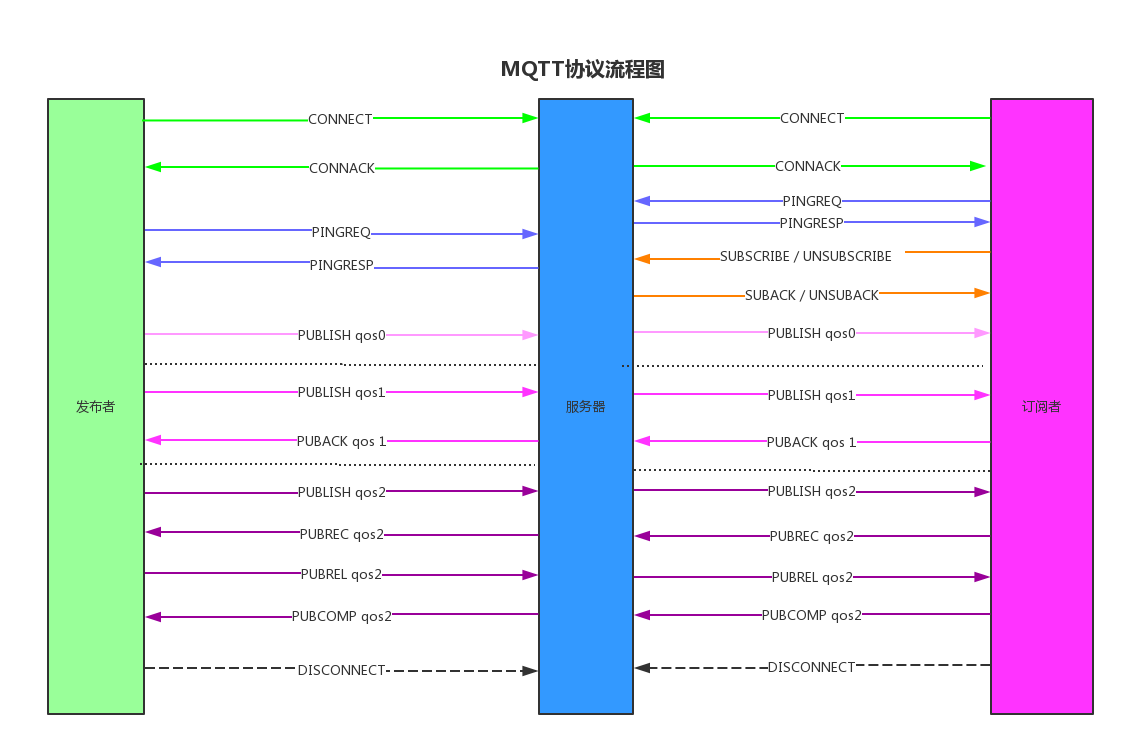
\includegraphics[width=1\linewidth]{figure/3-1}
	\caption{MQTT协议流程图}
	\label{fig:3-1}
\end{figure}


\subsection{关系性数据库 MySQL}


数据库(Database)是按照数据结构来组织、存储和管理数据的仓库。
每个数据库都有一个或多个不同的 API 用于创建,访问,管理,搜索和复制所保存的数据。
我们也可以将数据存储在文件中,但是在文件中读写数据速度相对较慢。
所以,现在我们使用关系型数据库管理系统(RDBMS)来存储和管理大数据量。所谓的关系型数据库,是建立在关系模型基础上的数据库,借助于集合代数等数学概念和方法来处理数据库中的数据。
\\RDBMS 即关系数据库管理系统(Relational Database Management System)的特点:

1.数据以表格的形式出现

2.每行为各种记录名称

3.每列为记录名称所对应的数据域

4.许多的行和列组成一张表单

5.若干的表单组成database


MySQL 是一个关系型数据库管理系统,由瑞典 MySQL AB 公司开发,目前属于 Oracle 公司。MySQL 是一种关联数据库管理系统,关联数据库将数据保存在不同的表中,而不是将所有数据放在一个大仓库内,这样就增加了速度并提高了灵活性。
MySQL具有以下特性:
\begin{itemize}
	\item MySQL 是开源的,目前隶属于 Oracle 旗下产品。
	\item MySQL 支持大型的数据库。可以处理拥有上千万条记录的大型数据库。
	\item MySQL 使用标准的 SQL 数据语言形式。
	\item MySQL 可以运行于多个系统上,并且支持多种语言。这些编程语言包括 C、C++、Python、Java、Perl、PHP、Eiffel、Ruby 和 Tcl 等。
	\item MySQL 支持大型数据库,支持 5000 万条记录的数据仓库,32 位系统表文件最大可支持 4GB,64 位系统支持最大的表文件为8TB。
	\item MySQL 是可以定制的,采用了 GPL 协议,你可以修改源码来开发自己的 MySQL 系统。
\end{itemize}

\subsection{Python开发语言 Flask模块}

Flask一直被称为是Python中轻量级的可定制的框架,其核心简单,相比其他框架更加灵活轻便,也更容易掌握。

你能Flask框架核心简单,同时在使用过程同样可以保持功能的丰富与扩展性,用户在使用Flask开发网站时,可以根据自己的需求添加不同的功能,各种强大的插件库可以让用户完全按照自己的意愿开发出功能强大的为国内站。

\begin{lstlisting}[title=代码 3-1:Flask简单示例]
from flask import Flask
app = Flask(__name__)
@app.route('/')
def index():
    return 'Hello World'
\end{lstlisting}

仅仅5行代码,就可以在浏览器中显示一个Hello World响应。所以Flask的其中一个优势再明显不过了:简洁。且不说Java的Web框架Spring,就说同样使用Python的框架Django,写一个Hello World程序也得10行代码。

第一行,导入包。

第二行,创建对象。

第三行,创建路由。

第四行、第五行,视图函数。

\subsection{SQLAlchemy---对象关系映射器(ORM)}

SQLAlchemy是一个功能非常强大的库,用于在Python中处理关系数据库。代替手工编写SQL查询,我们可以使用普通的Python对象来表示数据库表并执行查询。这种方法有很多好处,如下代码所示:

\begin{lstlisting}[title=DHT11数据表对象数据表模型]
class Dht11(PaginatedAPIMxin, db.Model):
__tablename__ = 'Dht11'
id = db.Column(db.Integer, primary_key=True)  #卡片存储收到MQTT数据的序号
temperature = db.Column(db.String(48), index=True) #存储MQTT数据中温度
humidity = db.Column(db.String(48), index=True)  #存储MQTT数据中湿度
timestamp = db.Column(db.DateTime, index=True, default=datetime.utcnow) #存储当前收到数据的时间戳
card_id = db.Column(db.Integer, db.ForeignKey('boards.id')) #对应的卡片ID

def __repr__(self):   #__repr__方法,它用于生成Dht11类实例的辅助显示内容
	return '<temp:{0}, humidity:{1}'.format(self.temperature, self.humidity)

def to_dict(self):  #单个对象方法
	data = {
		'id_from_db': self.id,
		'owner_email': str(User.query.get_or_404(self.card_id).email),
		'from_card_id': self.card_id,
		'value_created_at': self.timestamp,
		'temperature': self.temperature,
		'humidity': self.humidity,
		'_links': {
			(self.card_id).id) # user_id
			}
		}
	return data
\end{lstlisting}

通过ORM方法的使用很容易的构建了返回对象的数据格式

与手工编写SQL查询相反,我们可以使用普通的Python对象来表示数据库表,并执行查询。如下,该方法有很多的优点:

应用程序可以完全用Python开发。

数据库引擎之间的细微差别被抽象掉了。这使可以像处理轻量级数据库一样进行操作,例如,使用SQLite进行本地开发和测试,然后切换到专为生产中的高负载而设计的数据库(例如PostgreSQL)。

数据库错误不太常见,因为您的应用程序和数据库服务器之间现在存在两层:Python解释器本身(这将捕获明显的语法错误)和SQLAlchemy,后者具有定义良好的API和自己的错误检查层。

由于SQLAlchemy的工作单元模型有助于减少不必要的数据库往返次数,因此数据库代码可能会变得更加高效。SQLAlchemy还具有有效地预取相关对象的功能,称为预先加载。

对象关系映射(Object Relational Mapping,ORM)使代码更具可维护性,这被称为“不要重复自己”(DRY)。假设将列添加到模型中。使用SQLAlchemy,只要您使用该模型,它将可用。另一方面,如果整个应用程序中都散布着手写的SQL查询,则需要一次更新一次每个查询,以确保包含新列。SQLAlchemy可以帮助避免SQL注入漏洞。

出色的库支持:有很多有用的库可以直接与SQLAlchemy模型一起使用,以提供诸如维护接口和RESTful API之类的东西。

应用可以完全使用Python开发。


\subsection{RESTful 架构开发方式}
REST全称是Representational State Transfer,中文意思是表述(通常译为表现层状态转移)。 REST本身并没有创造新的技术、组件或服务,而隐藏在RESTful背后的理念就是使用Web的现有特征和能力, 更好地使用现有Web标准中的一些准则和约束。虽然REST本身受Web技术的影响很深, 但是理论上REST架构风格并不是绑定在HTTP上,只不过目前HTTP是唯一与REST相关的实例。 所以我这里描述的REST也是通过HTTP实现的REST。

REST全称是表述性状态转移,那究竟指的是什么的表述? 其实指的就是资源。任何事物,只要有被引用到的必要,它就是一个资源。资源可以是实体(例如手机号码),也可以只是一个抽象概念(例如价值) 。下面是一些资源的例子:
\\某用户的手机号码
\\某用户的个人信息

要让一个资源可以被识别,需要有个唯一标识,在Web中这个唯一标识就是URI(Uniform Resource Identifier)。

URI既可以看成是资源的地址,也可以看成是资源的名称。如果某些信息没有使用URI来表示,那它就不能算是一个资源, 只能算是资源的一些信息而已。URI的设计应该遵循可寻址性原则,具有自描述性,需要在形式上给人以直觉上的关联。这里以github网站为例,给出一些还算不错的URI:
https://github.com/git/git
https://github.com/git/git/blob/master/block-sha1/sha1.h
https://github.com/git/git/commit/e3af72cdafab5993d18fae056f87e1d675913d08
https://github.com/git/git/pulls
https://github.com/git/git/pulls?state=closed

1. REST描述的是在网络中client和server的一种交互形式;REST本身不实用,实用的是如何设计 RESTful API(REST风格的网络接口);
2. Server提供的RESTful API中,URL中只使用名词来指定资源,原则上不使用动词。“资源”是REST架构或者说整个网络处理的核心。
比如:
\begin{itemize}
	\item http://api.qc.com/v1/newsfeed: 获取某人的新鲜; 
	\item http://api.qc.com/v1/friends: 获取某人的好友列表;
	\item http://api.qc.com/v1/profile: 获取某人的详细信息;
\end{itemize}

3. 用HTTP协议里的动词来实现资源的添加,修改,删除等操作。即通过HTTP动词来实现资源的状态扭转:GET 用来获取资源,POST 用来新建资源(也可以用于更新资源),PUT 用来更新资源,DELETE 用来删除资源。比如:
\begin{itemize}
	\item DELETE http://api.qc.com/v1/friends: 删除某人的好友 (在http parameter指定好友id)
	\item GET  http://api.qc.com/v1/friends: 请求好友资料
	\item POST http://api.qc.com/v1/friends: 添加好友
	\item UPDATE http://api.qc.com/v1/profile: 更新个人资料
\end{itemize}

图例:
\begin{figure}[H]
	\centering
	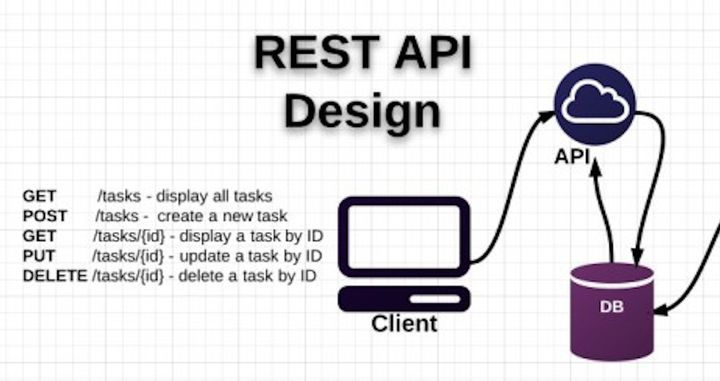
\includegraphics[width=0.85\linewidth]{figure/3-2}
	\caption{RESTful 设计理念图}
	\label{fig:3-2}
\end{figure}

通过使用RESTful可以做到:前后端分离,减少流量。
安全问题集中在接口上,由于接受json格式,防止了注入型等安全问题。
前端无关化,后端只负责数据处理,前端表现方式可以是任何前端语言(android,ios,html5)。
前端和后端人员更加专注于各自开发,只需接口文档便可完成前后端交互,无需过多相互了解。
服务器性能优化:由于前端是静态页面,通过nginx便可获取,服务器主要压力放在了接口上。
